
%\chapter*{A brief introduction to quantum field theory in curved spacetimes: Introduction to the Unruh and Hawking effects}[Intro to the Unruh and Hawking effects]
%\label{chap:introUnruh}

\chapter{Entanglement through the acceleration horizon\footnote{E. Mart\'in-Mart\'inez, J. Le\'on, Phys. Rev. A, 81, 032320 (2010)}}\label{etanthrough}


As thoroughly discussed in previous chapters, the Unruh effect degrades the entanglement between the two partners affecting all the quantum information tasks that they could perform. Specifically, it has been shown that, as Rob accelerates, entanglement is completely degraded for a scalar field \cite{Alicefalls} and, conversely, some degree of entanglement is preserved for fermionic fields. This behaviour of fermionic fields has been shown to be universal.  Namely, it is independent of  i) the spin of the fermionic field,  ii) the kind of maximally entangled state from which we start, and iii) the number of participating modes when studying a non-single mode state.

When Rob accelerates, the description of his partial state must be done by means of a basis built from solutions to the field equation in Rindler coordinates \cite{gravitation,Takagi}. As it will be shown below, the description of the system splits in three different subsystems; Alice's Minkowskian system, a subsystem in region I of Rindler spacetime (which we assign to Rob) and another subsystem, called AntiRob, constituted by the modes of the field in region $\text{II}$ of Rindler space time.

Any accelerated observer is constrained to either region I or $\text{II}$ of Rindler spacetime. If we select region I coordinates to account for the accelerated observer Rob, he would remain causally disconnected from region $\text{II}$, and therefore, Rob would be unable to communicate with the hypothetical observer AntiRob (who is accelerating with the same proper acceleration than Rob but decelerates with respect to the origin) in region $\text{II}$ as shown in Figure \ref{rar}.

\begin{figure}[h]
\begin{center}
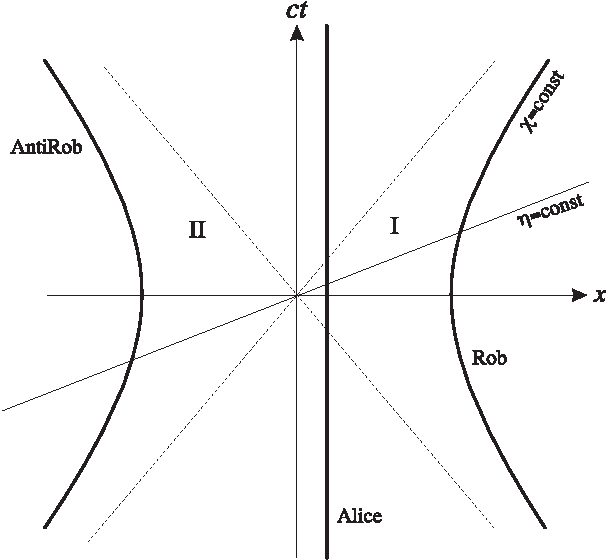
\includegraphics[width=.80\textwidth]{rar}
\end{center}
\caption{Flat spacetime. Trajectories of an inertial (Alice) and causally disconnected accelerated observers (Rob and AntiRob)}
\label{rar}
\end{figure}

To gain a deeper understanding of the entanglement degradation mechanisms it is useful to study how entanglement is lost as one traces over regions of the Rindler spacetime. Although the system is obviously bipartite (Alice and Rob), we saw that shifting to the Rindler basis for Rob the mathematical description of the system (\cite{Alicefalls,AlsingSchul} and previous chapters) admits a straightforward tripartition: Minkowskian modes (Alice), Rindler region I modes (Rob), and Rindler region $\text{II}$  modes (AntiRob). 

 Let us revisit the physical meaning  of each of
these three `observers'. Alice represents an observer in an inertial frame.
For Alice the states
\eqref{Min1} and \eqref{Minf} are maximally entangled.
Rob represents an accelerated observer moving in a $x=a^{-1}$
trajectory in Region I of Rindler spacetime (as seen in Fig. \ref{rar}) who shares a bipartite entangled state \eqref{Min1} or \eqref{Minf} with Alice.
AntiRob represents an observer  moving in a $x=a^{-1}$ trajectory in
Region II with access to the information to which Rob is not able to
access due to the presence of the Rindler horizon.

In this chapter, instead of considering only the Alice-Rob bipartition, we deal with all the different bipartitions of the system to study the correlation tradeoff among them. These three bipartitions are\begin{enumerate}
\item Alice-Rob $(\text{AR})$
\item Alice-AntiRob $(\text{A}{\bar{\text{R}}})$
\item Rob-AntiRob $(\text{R}{\bar{\text{R}}})$
\end{enumerate}

The first bipartition is the most commonly considered in the literature. It represents the system formed by an inertial observer and the modes of the field which an accelerated observer is able to access.

The second bipartition represents the subsystem formed by the inertial observer Alice and the modes of the field which Rob is not able to access due to the presence of an horizon as he accelerates.

The third bipartition lacks physical meaning in terms of information theory because communication between Rob and AntiRob is not allowed. Anyway, studying this bipartition is still useful to account for the correlations which are created between the spacetime regions separated by horizons and, therefore, its study is necessary and complementary to the previous ones in order to give a complete description of the information behaviour in non-inertial settings.

In \cite{AlsingSchul} the existence of these three possible bipartitions was considered only for spinless fermion fields. Bosonic fields were analysed in a completely different formalism (covariance matrices) in \cite{Adeschul} finding relationships between the correlations in both sides of the horizon. In this chapter we will go beyond previous analysis and we will compare the correlation tradeoff among different bipartitions for bosonic and fermionic fields in the standard formalism introduced before, showing the leading role of statistics in the behaviour of information in non-inertial frames. 

The work presented in this chapter will be useful to take a step in the discussion and refutation of the argument that the dimension of the Hilbert space is responsible for the difference between fermionic and bosonic entanglement behaviour in the presence of horizons. Indeed, we will present here an entanglement tradeoff between the bipartitions Alice-Rob and AliceAntiRob that only occurs for the fermionic case and that will reveal to be deeply connected with the fermionic entanglement survival in the limit $a\rightarrow\infty$.

\section{Scalar and Dirac fields from constantly accelerated frames}\label{sec2}

Following the standard conventions, let us denote the particle annihilation and creation operators in region I as $(a_{\omega,\text{I}}^{\phantom{\dagger}},a^{\dagger}_{\omega,\text{I}})$ for the scalar field  and $(c^{\phantom{\dagger}}_{\omega,s,\text{I}},c^{\dagger}_{\omega,s,\text{I}})$ for the Dirac field. $(d^{\phantom{\dagger}}_{\omega,s,\text{I}},d^{\dagger}_{\omega,s,\text{I}})$ are the corresponding antiparticle Dirac field operators. Analogously we define $(a^{\phantom{\dagger}}_{\omega\text{II}},a^{\dagger}_{\text{II},k})$, $(c^{\phantom{\dagger}}_{\omega,s,\text{II}},c^{\dagger}_{\omega,s,\text{II}})$, $(d^{\phantom{\dagger}}_{\omega,s,\text{II}},d_{\omega,s,\text{II}}^\dagger)$ as the particle/antiparticle operators in region \text{II}.

The bosonic operators satisfy the commutation relations $[a^{\phantom{\dagger}}_{\omega,\Sigma},a^\dagger_{\omega,\Sigma'}]=\delta_{\Sigma\Sigma'}\delta_{\omega\omega'}$. The fermionic ones satisfy  anticommutation relations $\{d^{\phantom{\dagger}}_{\omega,s,\Sigma},d^\dagger_{\omega',s',\Sigma'}\}=\delta_{\Sigma\Sigma'}\delta_{\omega\omega'}\delta_{ss'}$. The label $\Sigma$ notates the Rindler region of the operator  $\Sigma=\{\text{I},\text{II}\}$.  All other commutators and anticommutators are zero. This includes the anticommutators between operators in different Rindler regions.

We can relate Minkowski Unruh operators and Rindler creation and annihilation operators recalling the Bogoliubov relationships \eqref{buenmod}, \eqref{Bogoferm2}.

For a scalar field, the Bogoliubov relationships for the annihilation operator of modes with positive frequency are
\begin{equation}\label{bogoboson}
 a_{\omega,\text{U}}=\cosh r_\text{b}\, a_{\omega,\text{I}} - \sinh r_\text{b}\, a^\dagger_{\omega,\text{II}},
\end{equation}
where
\begin{equation}\label{defr1}
\tanh r_\text{b}=e^{-\pi \frac{\omega c}{a}}.
\end{equation}

For a Dirac field, the Bogoliubov relationships take the form
\begin{eqnarray}\label{bogodirac}
\nonumber c_{\omega,s,\text{U}}&=&\cos{r_\text{f}}\,c_{\omega,s,\text{I}}-\sin r_\text{f}\,d^\dagger_{\omega,-s,\text{II}}\\*
d^\dagger_{\omega,s,\text{U}}&=&\cos{r_\text{f}}\,d^\dagger_{\omega,s,\text{II}}+\sin r_\text{f}\,c_{\omega,-s,\text{I}},
\end{eqnarray}
where
\begin{equation}\label{defr2}
\tan r_\text{f}=e^{-\pi \frac{\omega c}{a}}.
\end{equation}

\section{Vacuum and one particle states}\label{sec3}

As it is shown in \cite{Alicefalls} and in previous chapters, the vacuum state of a scalar field as seen from the perspective of an accelerated observer is
\begin{equation}\label{scavac}
\ket{0}=\prod_{\omega}\frac{1}{\cosh r_\text{b}}\sum_{n=0}^\infty \tanh^n r_\text{b} \ket{n_\omega}_\text{I}\ket{n_{\omega}}_{\text{II}},
\end{equation}
and as it was discussed in previous chapters, the unprimed sector of the vacuum state for a Dirac field as seen from the accelerated frame is
\begin{equation}\label{diravac}
 \ket{0_\omega}=\cos^2 r_\text{f}\biketn{0}{0}+\sin r_\text{f}\cos r_\text{f}\left(\biketn{\uparrow}{\downarrow}+\biketn{\downarrow}{\uparrow}\right)+\sin^2 r_\text{f}\biketn{\pa}{\pa},
\end{equation}
where $\ket{\pa_\omega}^\pm$ represents the pair of particles/antiparticles of frequency $\omega$.

From now on we will drop the sign $\pm$ as as reasoned in section \ref{sec42m} a mode in region I will always be a particle mode and a mode in region $\text{II}$ will always represent an antiparticle mode. To simplify notation we will also drop the $\omega$ label as we focus on a single mode state.

As usual we will also need the Minkowskian Unruh one particle state in the Rindler basis which is obtained by applying $a^\dagger_{\text{U}}$ to the vacuum state. i.e. 
\begin{equation}
\ket{1}_\text{U}=\frac{1}{\cosh^2 r_\text{b}}\sum_{n=0}^\infty \tanh^n r_\text{b} \,\sqrt{n+1}\ket{n+1}_\text{I}\ket{n}_{\text{II}}
\end{equation} 	
for the scalar field \cite{Alicefalls} and 
\begin{eqnarray}\label{onepart2}
\nonumber\ket\uparrow_\text{U}&=&\cos r_\text{f} \biket{\uparrow}{0}+\sin r_\text{f}\biket{\pa}{\uparrow}\\*
\ket\downarrow_\text{U}&=&\cos r_\text{f} \biket{\downarrow}{0}-\sin r_\text{f}\biket{\pa}{\downarrow}
\end{eqnarray}
for the Dirac field (See chapter \ref{onehalf}).

Now we need to consider the following maximally entangled states in the Minkowski Unruh basis
\begin{eqnarray}
\label{entangledsca}\ket{\Psi_\text{b}}&=&\frac{1}{\sqrt{2}}\left(\ket{0}\ket{0}+\ket{1}_\text{U}\ket{1}_\text{U}\right),\\*
\label{entangleddir}\ket{\Psi_\text{f}}&=&\frac{1}{\sqrt{2}}\left(\ket{0}\ket{0}+\ket{\uparrow}_\text{U}\ket{\downarrow}_\text{U}\right).
\end{eqnarray}
These two maximally entangled states are analogous, both are bipartite qubit states superpositions of the vacuum and the one particle state. The difference is that in \eqref{entangleddir} we have a Dirac field state and hence, the one particle states have spin and follow fermionic statistics.

For $\ket{\Psi_\text{f}}$ we have selected one amongst the possible values for the spin of the terms with one particle for Alice and Rob, but it can be shown (see chapter \ref{onehalf}) that the choice of a specific value for these spins is not relevant when considering the behaviour of correlations. Then, the results presented here are independent of the particular choice of a spin state for the superposition \eqref{entangleddir}.



\section{Correlations for the Dirac field}\label{sec4m4}

The density matrix for the whole tripartite state, which includes modes on both sides of the Rindler horizon along with Minkowskian modes, is built from \eqref{entangleddir}
\begin{equation}\label{tripadir}
\rho^{A\text{R}{\bar{\text{R}}}}_\text{f}=\proj{\Psi_\text{f}}{\Psi_\text{f}}.
\end{equation}

The three different bipartite partial density matrices are obtained by partial tracing:
\begin{eqnarray}
\label{AR2}\rho^\text{AR}_\text{f}&\!\!=\!&\tr_{\text{II}}\rho^{A\text{R}{\bar{\text{R}}}}_\text{f}=\!\!\!\!\sum_{s\in\{0,\uparrow,\downarrow,\pa\}} \bra{s}_{\text{II}}\rho_\text{f}^{A\text{R}{\bar{\text{R}}}}\ket{s}_{\text{II}},\\*
\label{AAR2}\rho^{\text{A}{\bar{\text{R}}}}_\text{f}&\!\!=\!&\tr_\text{I}\rho^{A\text{R}{\bar{\text{R}}}}_\text{f}=\!\!\!\!\sum_{s\in\{0,\uparrow,\downarrow,\pa\}} \bra{s}_\text{I}\rho_\text{f}^{A\text{R}{\bar{\text{R}}}}\ket{s}_\text{I},\\*
\label{RAR2}\rho^{\text{R}{\bar{\text{R}}}}_\text{f}&\!\!=\!&\tr_\text{U}\rho^{A\text{R}{\bar{\text{R}}}}_\text{f}=\!\!\!\!\sum_{s\in\{0,\uparrow,\downarrow,\pa\}} \bra{s}_\text{U}\rho_\text{f}^{A\text{R}{\bar{\text{R}}}}\ket{s}_\text{U},
\end{eqnarray}
and the density matrix for each individual subsystem is obtained by tracing over the other subsystems,
 \begin{eqnarray}
\label{A2}\rho^{\text{A}}_\text{f}&=&\tr_\text{I}\rho^\text{AR}_\text{f}=\tr_{\text{II}}\rho^{\text{A}{\bar{\text{R}}}}_\text{f},\\*
\label{R2}\rho^{\text{R}}_\text{f}&=&\tr_{\text{II}}\rho^{\text{R}{\bar{\text{R}}}}_\text{f}=\tr_\text{U}\rho^\text{AR}_\text{f},\\*
\label{aR2}\rho^{{\bar{\text{R}}}}_\text{f}&=&\tr_\text{I}\rho^{\text{R}{\bar{\text{R}}}}_\text{f}=\tr_\text{U}\rho^{\text{A}{\bar{\text{R}}}}_\text{f}.
\end{eqnarray}
In the cases AR and $\text{A}\bar{\text{R}}$, there are physical
arguments to justify the need for the partial trace beyond mere
quantum information considerations. Namely, Rob will never be  able to
access region II of the spacetime due to the presence of the Rindler
horizon so that $\bar{\text{R}}$ (Region $\text{II}$) must be traced
out. Likewise, AntiRob is not able to access region I  because of the
horizon and hence R (Region I) must be traced out. For the subsystem
${\text{R}\bar{\text{R}}}$ taking the partial trace over subsystem A corresponds
to the standard procedure for analysing correlations between two parts
of a multipartite system. 


The different bipartitions are characterised by the following density matrices
\begin{align}\label{rhoars2}
\nonumber \rho^\text{AR}_\text{f}&=\frac12\Big[\cos^4 r_\text{f} \proj{00}{00}+\sin^2 r_\text{f}\,\cos^2 r_\text{f}\Big(\proj{0\uparrow}{0\uparrow}+\proj{0\downarrow}{0\downarrow}\Big)+\sin^4 r_\text{f}\proj{0\pa}{0\pa}\\
&+\cos^3r_\text{f}\Big(\ket{00}\bra{\uparrow\downarrow}  +\proj{\uparrow\downarrow}{00}\Big)-\sin^2 r_\text{f}\cos r_\text{f}\Big(\proj{0\uparrow}{\uparrow\pa}+\proj{\uparrow\pa}{0\uparrow}\Big)\nonumber\\*
& +\cos^2 r_\text{f} \proj{\uparrow\downarrow}{\uparrow\downarrow}+\sin^2 r_\text{f}\proj{\uparrow\pa}{\uparrow\pa}\Big],
\end{align}
\begin{align}\label{rhoa-rs2}
\nonumber \rho^{\text{A}{\bar{\text{R}}}}_\text{f}&=\frac12\Big[\cos^4 r_\text{f} \proj{00}{00}+\sin^2 r_\text{f}\,\cos^2 r_\text{f}\Big(\proj{0\downarrow}{0\downarrow}+\proj{0\uparrow}{0\uparrow}\Big)+\sin^4 r_\text{f}\proj{0\pa}{0\pa} \nonumber\\*
& -\sin^3r_\text{f}\Big(\proj{0\pa}{\uparrow\downarrow}+\proj{\uparrow\downarrow}{0\pa}\Big)+\sin r_\text{f}\cos^2 r_\text{f}\Big(\ket{0\uparrow}\bra{\uparrow0}+\proj{\uparrow0}{0\uparrow}\Big)\nonumber\\*
&+\cos^2 r_\text{f} \proj{\uparrow0}{\uparrow0}+\sin^2 r_\text{f}\proj{\uparrow\downarrow}{\uparrow\downarrow}\Big],
\end{align}
\begin{align}\label{rhor-rs2}
\nonumber \rho^{\text{R}{\bar{\text{R}}}}_\text{f}&=\frac{1}{2}\Big[\cos^4 r_\text{f} \proj{00}{00}+\sin r_\text{f}\, \cos^3 r_\text{f}\Big(\proj{00}{\uparrow\downarrow}+\ket{00}\bra{\downarrow\uparrow}+\proj{\uparrow\downarrow}{00}+\proj{\downarrow\uparrow}{00}\Big)\\*
&\nonumber +\sin^2 r_\text{f}\cos^2 r_\text{f}\Big(\ket{00}\bra{\pa\pa}\!+\!\proj{\uparrow\downarrow}{\uparrow\downarrow}\!+\!\proj{\uparrow\downarrow}{\downarrow\uparrow}\!+\!\proj{\downarrow\uparrow}{\uparrow\downarrow}\!+\!\proj{\downarrow\uparrow}{\downarrow\uparrow}+\proj{\pa\pa}{00}\Big)\\*
&\nonumber + \sin^3 r_\text{f}\,\cos r_\text{f}\Big(\proj{\uparrow\downarrow}{\pa\pa}+\proj{\pa\pa}{\uparrow\downarrow}+\ket{\downarrow\uparrow}\bra{\pa\pa}\!+\!\proj{\pa\pa}{\downarrow\uparrow}\Big)+\cos^2 r_\text{f}\proj{\downarrow 0}{\downarrow 0}\\*
&\nonumber+\sin^2 r_\text{f}\proj{\pa\downarrow}{\pa\downarrow}-\cos r_\text{f}\,\sin r_\text{f}\Big(\proj{\downarrow0}{\pa\downarrow}+\ket{\pa\downarrow}\bra{\downarrow0}\Big)+\sin^4r_\text{f}\proj{\pa\pa}{\pa\pa}\Big],\\*
\end{align}
where the bases are
\begin{eqnarray}\label{barbolbasis2}
 \ket{nm}&=&\ket{n^\text{A}}_\text{U}\ket{m^\text{R}}_\text{I},\\*
\ket{nm}&=&\ket{n^\text{A}}_\text{U}|m^{{\bar{\text{R}}}}\rangle_{\text{II}},\\*
\ket{nm}&=&\ket{n^\text{R}}_\text{I}|m^{{\bar{\text{R}}}}\rangle_{\text{II}}
\end{eqnarray}
respectively for \eqref{rhoars2}, \eqref{rhoa-rs2} and \eqref{rhor-rs2}.

On the other hand, the density matrices for the individual subsystems \eqref{A2}, \eqref{R2},\eqref{aR2} are
\begin{align}\label{robfpartialstate}
\nonumber \rho^{\text{R}}_\text{f}&=\frac12\Big[\sin^2r_\text{f}(1+\sin^2 r_\text{f})\proj{\pa}{\pa}+\sin^2 r_\text{f}\cos^2r_\text{f}\proj{\uparrow}{\uparrow}+\cos^2 r_\text{f}(1+\sin^2 r_\text{f})\proj{\downarrow}{\downarrow}\\*
&+\cos^4r_\text{f}\proj{0}{0}\Big],
\end{align}
\begin{align}\label{arobfpartialstate}
\nonumber \rho^{{\bar{\text{R}}}}_\text{f}&=\frac12\Big[\cos^2r_\text{f}(1+\cos^2r_\text{f})\proj{0}{0}+\sin^2 r_\text{f}\cos^2r_\text{f}\proj{\uparrow}{\uparrow}+\sin^2 r_\text{f}(1+\cos^2 r_\text{f})\proj{\downarrow}{\downarrow}\\*&+\sin^4r_\text{f}\proj{\pa}{\pa}\Big],
\end{align}
\begin{equation}\label{alicefpartialstate}
 \rho^{\text{A}}_\text{f}=\frac12\left(\proj{0}{0}+\proj{\uparrow}{\uparrow}\right).
\end{equation}

\subsection{Mutual Information: creation, exchange and conservation}

In this section we will compute mutual information (see section \ref{mutusec}) which accounts for correlations (both quantum and classical) between two different parts of a system. It is defined as
\begin{equation}\label{mutualdef}
I_{AB}=S_A+S_B-S_{AB},
\end{equation}
where $S_A$, $S_B$ and $S_{AB}$ are respectively the Von Neuman entropies for the individual subsystems $A$ and $B$ and for the joint system $AB$.

To compute the mutual information  for each bipartition we will need the eigenvalues of the corresponding density matrices. We shall go through all the process step by step in the lines below.

\subsubsection{Bipartition Alice-Rob}

The eigenvalues of the matrix for the system Alice-Rob \eqref{rhoars2} are
\begin{eqnarray}\label{eigAR4m1}
\nonumber \lambda_1&=&\lambda_2=0,\\*
\nonumber \lambda_3&=&\frac12\sin^2r_\text{f}\cos^2r_\text{f},\\*
\nonumber \lambda_4&=&\frac12\sin^4r_\text{f},\\*
\nonumber \lambda_5&=&\frac12\cos^2r_\text{f}\left(1+\cos^2r_\text{f}\right),\\*
\lambda_6&=&\frac12\sin^2r_\text{f}\left(1+\cos^2r_\text{f}\right).
\end{eqnarray}

\subsubsection{Bipartition Alice-AntiRob}

The eigenvalues of the matrix for the system Alice-AntiRob \eqref{rhoa-rs2} are
\begin{eqnarray}\label{eigAaR4m1}
\nonumber \lambda_1&=&\lambda_2=0,\\*
\nonumber \lambda_3&=&\frac12\sin^2r_\text{f}\cos^2 r_\text{f},\\*
\nonumber \lambda_4&=&\frac12\cos^4 r_\text{f},\\*
\nonumber \lambda_5&=&\frac12\sin^2r_\text{f} \left(1+\sin^2 r_\text{f}\right),\\*
 \lambda_6&=&\frac12\cos^2 r_\text{f}\left(1+\sin^2 r_\text{f}\right).
\end{eqnarray}

\subsubsection{Bipartition Rob-AntiRob}

All the eigenvalues of the matrix for the system Rob-AntiRob \eqref{rhor-rs2} are zero excepting two of them
\begin{equation}\label{eigRaR4m1}
\lambda_1=\lambda_2=\frac12,\qquad \lambda_{i>2}=0.
\end{equation}

\subsubsection{Von Neumann entropies for each subsystem and mutual information}

To compute the Von Neumann entropies we need the eigenvalues of every bipartition and the individual density matrices. The eigenvalues of $\rho^\text{AR}_\text{f}$, $\rho^{\text{A}{\bar{\text{R}}}}_\text{f}$, $\rho^{\text{R}{\bar{\text{R}}}}_\text{f}$ are respectively \eqref{eigAR4m1}, \eqref{eigAaR4m1} and \eqref{eigRaR4m1}.

The eigevalues of the individual systems density matrices can be directly read from \eqref{robfpartialstate}, \eqref{arobfpartialstate} and \eqref{alicefpartialstate} since $\rho^\text{R}_\text{b}$, $\rho^{{\bar{\text{R}}}}_\text{b}$ and $\rho^\text{A}_\text{b}$ have diagonal forms in the given basis.

The Von Neumann entropy for a partition $B$ of the system is
\begin{equation}\label{Vonneu}
S_B=-\tr(\rho\log_2 \rho)=-\sum \lambda_\text{I}\log_2\lambda_\text{I}.
\end{equation}

At this point, computing the entropies is quite straightforward. The Von Neumann entropies for all the partial systems are
\begin{align}
\nonumber S_R&=1-\sin^2r_\text{f}\log_2(\sin^2r_\text{f})-\frac32\cos^2r_\text{f}\log_2(\cos^2r_\text{f})-\frac{1+\sin^2r_\text{f}}{2}\log_2(1+\sin^2r_\text{f}),\\*
\nonumber S_{\bar R}&=1-\cos^2r_\text{f}\log_2(\cos^2r_\text{f})-\frac32\sin^2r_\text{f}\log_2(\sin^2r_\text{f})-\frac{1+\cos^2r_\text{f}}{2}\log_2(1+\cos^2r_\text{f}),
\end{align}
\begin{equation}
 S_{AR}=S_{\bar R}; \qquad S_{\text{A}{\bar{\text{R}}}}=S_{R}; \qquad S_{R\bar R}=S_{A}=1.
 \end{equation}


And then, the mutual information for all the possible bipartitions of the system will be
\begin{eqnarray}
\nonumber I_{AR}&=&S_A+S_R-S_{A R}=1+S_R -S_{\bar R},\\*
\nonumber I_{\text{A}{\bar{\text{R}}}}&=&S_A+S_{\bar R}-S_{\text{A}{\bar{\text{R}}}}=1+ S_{\bar R}-S_R,\\*
\nonumber I_{R\bar R}&=& S_R+S_{\bar R}-S_{R\bar R}=S_R+S_{\bar R}-1.
\end{eqnarray}  
At first glance we see a conservation law for the mutual information for the system Alice-Rob and Alice-AntiRob
\begin{equation}\label{conservation1}
 I_{AR} + I_{\text{A}{\bar{\text{R}}}}=2,
\end{equation}
which suggests a correlation transfer from the system Alice-Rob to Alice-AntiRob as the acceleration increases.

Fig. \ref{mutuferm} shows the behaviour of the mutual information for the three bipartitions. It also shows how the correlations across the horizon (Rob and AntiRob) increase, up to certain finite limit, as Rob accelerates. 

If we recall the results on spinless fermion fields \cite{AlsingSchul} we see that the conservation law obtained here is also valid for that spinless fermion case. This result was expected according to the universality argument stated  in the previous chapter.

However, something different occurs with the system Rob-AntiRob. The creation of correlations between modes on both sides of the horizon is greater in the Dirac field case. One have to be careful interpreting this result since the negativity entropy upper bound is a function of the dimension of the Hilbert space. The  fermionic field has a finite upper limit. For bosons the unbounded dimension of the Hilbert space implies that negativity can grow unboundedly. In principle this does not guarantee that one can extract more information from bosons than from fermions, even more when we are concerned about correlations between Rob and Anti-Rob that cannot communicate with each other.
\begin{figure}[h]
\begin{center}
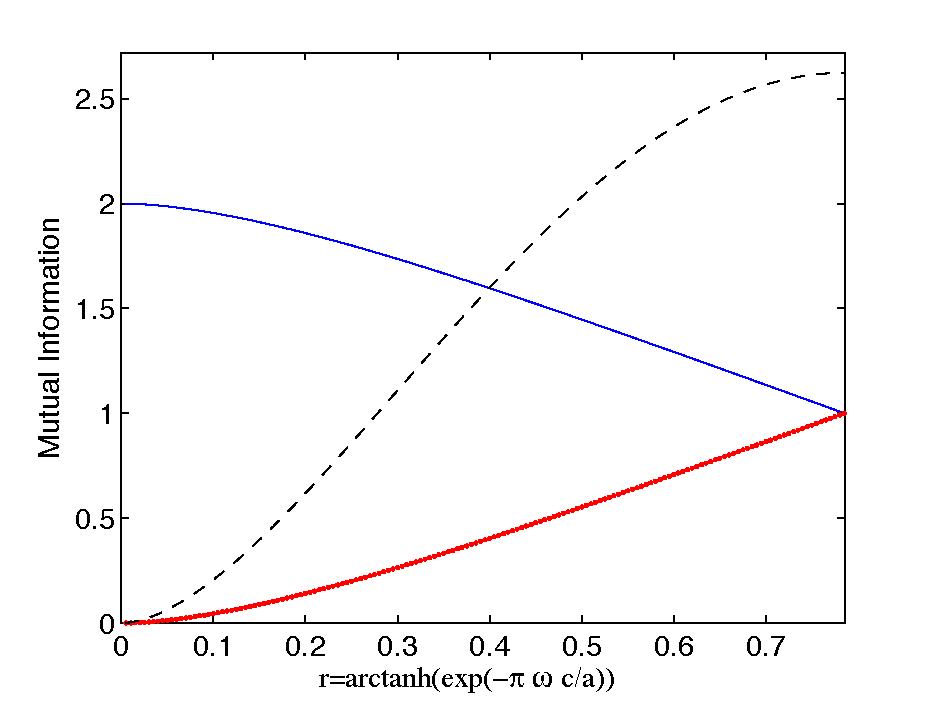
\includegraphics[width=.85\textwidth]{mutuferm}
\end{center}
\caption{ Dirac field: Mutual information tradeoff and conservation law between the systems Alice-Rob and Alice-AntiRob as acceleration varies. It is also shown the behaviour of the mutual information for the system Rob-AntiRob. Blue continuous line: Mutual information $AR$, red dotted line: Mutual information $\text{A}{\bar{\text{R}}}$, black dashed line: Mutual information $R\bar R$.}
\label{mutuferm}
\end{figure}

\subsection{Entanglement conservation and behaviour across the Rindler horizon}\label{conservanet}

To compute the negativity, we will need the partial transpose of the bipartite density matrices \eqref{rhoars2}, \eqref{rhoa-rs2} and \eqref{rhor-rs2}, which we will notate as $\eta^\text{AR}_\text{f}$, $\eta^{\text{A}{\bar{\text{R}}}}_\text{f}$ and $\eta^{\text{R}{\bar{\text{R}}}}_\text{f}$  respectively.

\begin{align}\label{etaARd}
\nonumber\eta^\text{AR}_\text{f}&=\frac12\Big[\cos^4r_\text{f}\proj{00}{00}+\sin^2r_\text{f}\cos^2r_\text{f}\left(\proj{0\uparrow}{0\uparrow}+\proj{0\downarrow}{0\downarrow}\right)+\sin^4r_\text{f}\proj{0\pa}{0\pa}\\*
\nonumber&+\cos^3r_\text{f}\left(\proj{0\downarrow}{\uparrow0}+\proj{\uparrow0}{0\downarrow}\right)-\sin^2r_\text{f}\,\cos r_\text{f}\left(\proj{0\pa}{\uparrow\uparrow}+\proj{\uparrow\uparrow}{0\pa}\right)\\*
&+\cos^2r_\text{f}\proj{\uparrow\downarrow}{\uparrow\downarrow}+\sin^2r_\text{f}\proj{\uparrow\pa}{\uparrow\pa}\Big],
\end{align}
\begin{align}\label{etaAaRd}
\nonumber \eta^{\text{A}{\bar{\text{R}}}}_\text{f}&=\frac12\Big[\cos^4 r_\text{f} \proj{00}{00}+\sin^2 r_\text{f}\cos^2 r_\text{f}\Big(\proj{0\downarrow}{0\downarrow}+\proj{0\uparrow}{0\uparrow}\Big)+\sin^4 r_\text{f}\proj{0\pa}{0\pa} \nonumber\\*
& -\sin^3r_\text{f}\Big(\proj{0\downarrow}{\uparrow\pa}+\proj{\uparrow\pa}{0\downarrow}\Big)+\sin r_\text{f}\cos^2 r_\text{f}\nonumber\Big(\ket{00}\bra{\uparrow\uparrow}+\proj{\uparrow\uparrow}{00}\Big)\nonumber\\*
&+\cos^2 r_\text{f} \proj{\uparrow0}{\uparrow0}+\sin^2 r_\text{f}\proj{\uparrow\downarrow}{\uparrow\downarrow}\Big],
\end{align}
\begin{align}\label{etaRaRd}
\nonumber \eta^{\text{R}{\bar{\text{R}}}}_\text{f}&\!=\!\frac{1}{2}\Big[\cos^4 r_\text{f} \proj{00}{00}\!+\!\sin r_\text{f} \cos^3 r_\text{f}\Big(\proj{0\!\downarrow}{\uparrow\! 0}\!+\!\ket{0\!\uparrow} \bra{\downarrow\! 0}\!+\!\proj{\uparrow 0}{0 \downarrow}\!+\!\proj{\downarrow\! 0}{0\!\uparrow}\Big)\\*
&\nonumber+\sin^2 r_\text{f} \cos^2 r_\text{f}\Big(\ket{0\pa}\bra{\pa0}\!+\!\proj{\uparrow\downarrow}{\uparrow\downarrow}\!+\!\proj{\uparrow\uparrow}{\downarrow\downarrow} +\proj{\downarrow\downarrow}{\uparrow\uparrow}+\proj{\downarrow\uparrow}{\downarrow\uparrow}+\proj{\pa0}{0\pa}\Big)\\*
&\nonumber\!+\! \sin^3 r_\text{f}\cos r_\text{f}\Big(\proj{\uparrow\!\pa}{\pa\!\downarrow}\!+\!\proj{\pa\!\downarrow}{\uparrow\!\pa}\!+\!\ket{\downarrow\!\pa}\bra{\pa\!\uparrow}\!+\!\proj{\pa\!\uparrow}{\downarrow\!\pa}\Big)\!+\!\cos^2 r_\text{f}\proj{\downarrow\! 0}{\downarrow\! 0}\\*
&+\sin^2 r_\text{f} \ket{\pa\downarrow} \bra{\pa\downarrow}-\cos r_\text{f}\,\sin r_\text{f}\Big(\proj{\downarrow\downarrow}{\pa0}+\ket{\pa0}\bra{\downarrow\downarrow}\Big)+\sin^4r_\text{f}\proj{\pa\pa}{\pa\pa}\Big].
\end{align}

In the following paragraphs we shall compute the negativity for each bipartition of the system.
 
\subsubsection{Bipartition Alice-Rob}

The non-positive eigenvalues of the partial transpose density matrix  for the bipartition Alice-Rob \eqref{etaARd} are
\begin{align}\label{eigetaARf}
\nonumber \lambda_{1}&=\frac14\sin^2 r_\text{f}\cos^2 r_\text{f}\left(1-\sqrt{1+\frac{4\cos^2 r_\text{f}}{\sin^4 r}}\right),\\*
 \lambda_{2}&=\frac14\sin^4 r_\text{f}\left(1-\sqrt{1+\frac{4\cos^2 r_\text{f}}{\sin^4 r_\text{f}}}\right).
\end{align}
The negativity, after some basic algebra turns out to be
\begin{equation}
\mathcal{N}_\text{f}^\text{AR}=\frac12\cos^2r_\text{f}.
\end{equation}

\subsubsection{Bipartition Alice-AntiRob}

The non-positive eigenvalues of the partial transpose density matrix for the bipartition Alice-AntiRob \eqref{etaAaRd} are
\begin{eqnarray}\label{eigetaAaRf}
\nonumber \lambda_{1}&=&\frac14\sin^2 r_\text{f}\cos^2 r_\text{f}\left(1-\sqrt{1+\frac{4\tan^2 r_\text{f}}{\cos^2 r_\text{f}}}\right),\\*
\lambda_{2}&=&\frac14\cos^4 r_\text{f}\left(1-\sqrt{1+\frac{4\tan^2 r_\text{f}}{\cos^2 r_\text{f}}}\right).
\end{eqnarray}
The negativity yields in this case
%\begin{equation}
%\mathcal{N}^{\text{A}{\bar{\text{R}}}}_\text{f}=\frac14\cos^2 r_\text{f}\left(\sqrt{1+\frac{4\tan^2 r_\text{f}}{\cos^2 r_\text{f}}}-1\right)
%\end{equation}
%which after some basic algebra results into the simple expression
\begin{equation}
\mathcal{N}^{\text{A}{\bar{\text{R}}}}_\text{f}=\frac12\sin^2 r_\text{f}.\end{equation}

It is remarkable --and constitutes one of the most suggestive results of this chapter-- that we have obtained here a conservation law for the entanglement Alice-Rob and Alice-AntiRob, since the sum of both negativities is independent of the acceleration
\begin{equation}\label{conservationN}
\mathcal{N}^{\text{A}{\bar{\text{R}}}}_\text{f} +\mathcal{N}_\text{f}^\text{AR} =\frac12.
\end{equation}
This is similar to the result \eqref{conservation1} for mutual information. Again, one could check that for spinless fermion fields the same  conservation law \eqref{conservationN} obtained here applies. This was again expected due to the universality principle exposed in previous chapters.

As we will see below, this is a genuine statistical effect: this conservation of quantum correlations is exclusive of fermionic fields and nothing of the sort will be found for bosonic fields. 


For the bipartition Rob-AntiRob the expression for the negativity is not as simple as it was for the previous cases, this negativity is plotted in Fig. \ref{negaferm}. We can see that the entanglement between Rob and AntiRob, created as Rob accelerates, grows up to a finite value. Although this entanglement is useless for quantum information tasks because of the impossibility of classical communication between both sides of an event horizon, the result obtained here may be a useful hint in order to understand how information behaves in the proximity of horizons.

Comparing again this result with spinless fermions \cite{AlsingSchul}, we see that for Dirac fields, the maximum value of the negativity is greater. Again this is strongly related with the dimension of the Hilbert space\footnote{For the Dirac case correlations between the the spin-up mode for Rob and the spin-down mode for AntiRob show up as well, even though the spin-up mode was not excited in \eqref{entangleddir}. This phenomenon cannot happen for the Grassmann scalar case where there is no spin.} that imposes a bound in negativity as mentioned before.
\begin{figure}[h]
\begin{center}
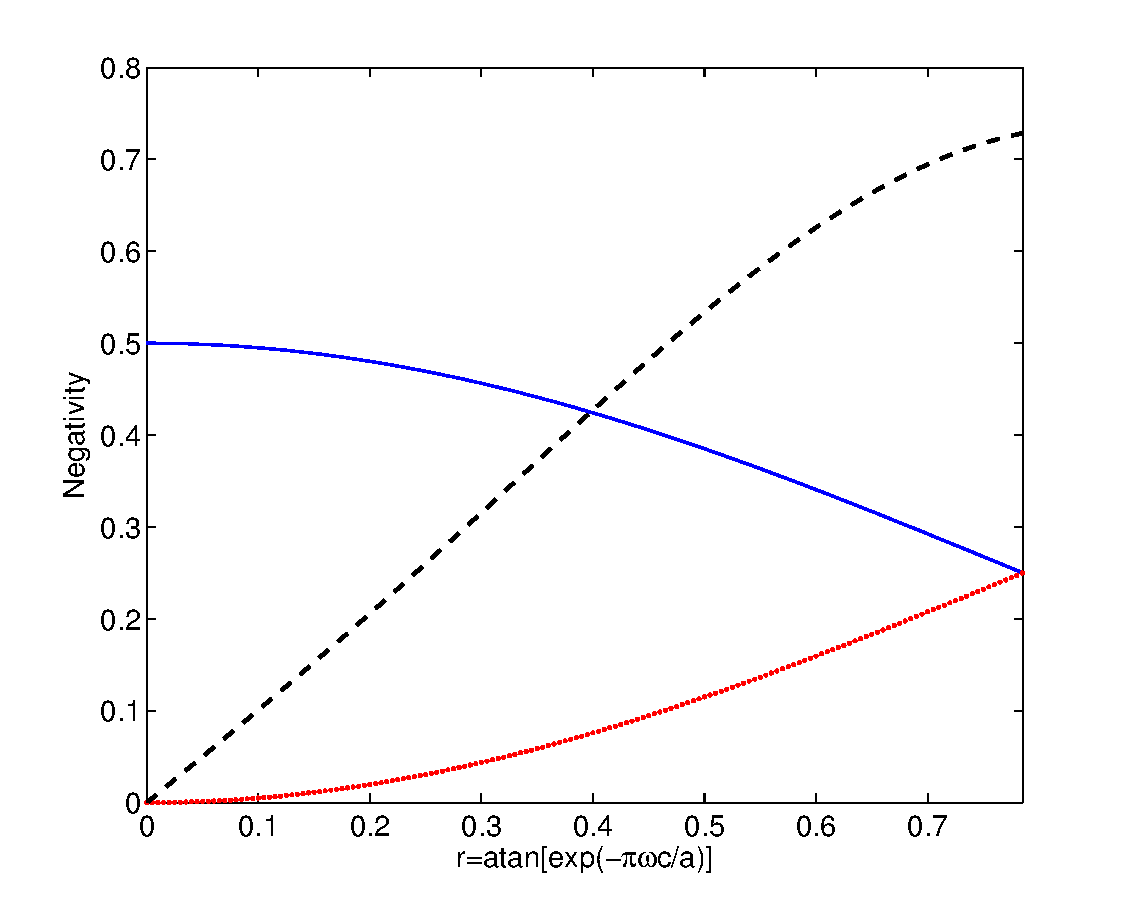
\includegraphics[width=.85\textwidth]{negaferm}
\end{center}
\caption{ Dirac field: Negativity tradeoff and conservation law between the systems Alice-Rob and Alice-AntiRob  as acceleration varies. It is also shown the behaviour of the quantum correlations for the system Rob-AntiRob. Blue continuous line: Negativity $AR$, red dotted line: Negativity $\text{A}{\bar{\text{R}}}$, black dashed line: Negativity $R\bar R$ }
\label{negaferm}
\end{figure}




\section{Correlations for the scalar field}\label{sec5}

The density matrix for the whole tripartite state, which includes modes in both sides of the horizon along with Minkowskian modes, is built from \eqref{entangledsca}
\begin{equation}\label{tripasca}
\rho^{A\text{R}{\bar{\text{R}}}}_\text{b}=\proj{\Psi_\text{b}}{\Psi_\text{b}}.
\end{equation}

As in the fermion case, the three different bipartitions for the scalar field case are obtained as follows
\begin{eqnarray}
\label{AR1}\rho^\text{AR}_\text{b}&=&\tr_{\text{II}}\rho^{A\text{R}{\bar{\text{R}}}}_\text{b},\\*
\label{AAR1}\rho^{\text{A}{\bar{\text{R}}}}_\text{b}&=&\tr_\text{I}\rho^{A\text{R}{\bar{\text{R}}}}_\text{b},\\*
\label{RAR1}\rho^{\text{R}{\bar{\text{R}}}}_\text{b}&=&\tr_\text{U}\rho^{A\text{R}{\bar{\text{R}}}}_\text{b}.
\end{eqnarray}
and the density matrix for each individual subsystem
 \begin{eqnarray}
\label{A1}\rho^{\text{A}}_\text{b}&=&\tr_\text{I}\rho^\text{AR}_\text{b}=\tr_{\text{II}}\rho^{\text{A}{\bar{\text{R}}}}_\text{b},\\*
\label{R1}\rho^{\text{R}}_\text{b}&=&\tr_{\text{II}}\rho^{\text{R}{\bar{\text{R}}}}_\text{b}=\tr_\text{U}\rho^\text{AR}_\text{b},\\*
\label{aR1}\rho^{{\bar{\text{R}}}}_\text{b}&=&\tr_\text{I}\rho^{\text{R}{\bar{\text{R}}}}_\text{b}=\tr_\text{U}\rho^{\text{A}{\bar{\text{R}}}}_\text{b}.
\end{eqnarray}

The bipartite systems are characterised by the following density matrices
\begin{align}\label{rhoars14m}
\nonumber\rho^\text{AR}_\text{b}&=\sum_{n=0}^{\infty}\frac{\tanh^{2n}r_\text{b}}{2\cosh^2 r_\text{b}}\Big[\proj{0n}{0n}+\frac{\sqrt{n+1}}{\cosh r_\text{b}}\Big(\proj{0n}{1\, n+1}+\proj{1\, n+1}{0n}\Big)\\*
&+\frac{n+1}{\cosh^2 r_\text{b}}\proj{1\,n+1}{1\,n+1}\Big],
\end{align}
\begin{align}\label{rhoa-rs14m}
\nonumber\rho^{\text{A}{\bar{\text{R}}}}_\text{b}&=\sum_{n=0}^{\infty}\frac{\tanh^{2n}r_\text{b}}{2\cosh^2 r_\text{b}}\Big[\!\proj{0n}{0n}\!+\!\frac{\sqrt{n+1}}{\cosh r_\text{b}}\tanh r_\text{b}\Big(\!\ket{0\,n+1}\times\bra{1 n}+\proj{1 n}{0\,n+1}\Big),\\*
&+\frac{n+1}{\cosh^2 r_\text{b}}\proj{1n}{1n}\Big].
\end{align}
\begin{align}\label{rhor-rs14m}
\rho^{\text{R}{\bar{\text{R}}}}_\text{b}&=\sum_{\substack{n=0\\m=0}}^{\infty}\frac{\tanh^{n+m}r_\text{b}}{2\cosh^2 r_\text{b}}\Big(\proj{nn}{mm}+\frac{\sqrt{n+1}\sqrt{m+1}}{\cosh^2 r_\text{b}}\times\proj{n+1\,n}{m+1\,m}\!\Big),
\end{align}
where the bases are respectively
\begin{eqnarray}\label{barbolbasis}
 \ket{nm}&=&\ket{n^\text{A}}_\text{U}\ket{m^\text{R}}_\text{I},\\*
\ket{nm}&=&\ket{n^\text{A}}_\text{U}|m^{{\bar{\text{R}}}}\rangle_{\text{II}},\\*
\ket{nm}&=&\ket{n^\text{R}}_\text{I}|m^{{\bar{\text{R}}}}\rangle_{\text{II}}
\end{eqnarray}
for \eqref{rhoars14m}, \eqref{rhoa-rs14m} and \eqref{rhor-rs14m}.

On the other hand, the density matrices for the individual subsystems \eqref{A1}, \eqref{R1},\eqref{aR1} are
\begin{equation}\label{Robpartialm4}
\rho^{\text{R}}_\text{b}=\sum_{n=0}^\infty\frac{\tanh^{2(n-1)}r_\text{b}}{2\cosh^2 r_\text{b}}\left[\tanh^2 r_\text{b}+\frac{n}{\cosh^2r_\text{b}}\right]\proj{n}{n},
\end{equation}
\begin{equation}\label{ARobpartialm4}
\rho^{{\bar{\text{R}}}}_\text{b}=\sum_{n=0}^\infty\frac{\tanh^{2n}r_\text{b}}{2\cosh^2 r_\text{b}}\left[1+\frac{n+1}{\cosh^2r_\text{b}}\right]\proj{n}{n},
\end{equation}
\begin{equation}\label{AlicedeAliceRobm4}
\rho^{\text{A}}_\text{b}=\frac12\left(\proj{0}{0}+\proj{1}{1}\right).
\end{equation}

\subsection{Mutual Information: creation, exchange and conservation}


To compute the mutual information  for each bipartition we need the eigenvalues of the corresponding density matrices. We shall go through all the process in detail in the lines below.

\subsubsection{Bipartition Alice-Rob}

The density matrix for the system Alice-Rob \eqref{rhoars14m}  consists on an infinite number of $2\times2$ blocks in the basis $\{\ket{0 n},\ket{1\, n+1}\}_{n=0}^\infty$ which have the form
\begin{equation}
\frac{\tanh^{2n}r_\text{b}}{2\cosh^2 r_\text{b}}
\left(\!\begin{array}{cc}
1 & \dfrac{\sqrt{n+1}}{\cosh r_\text{b}}\\
\dfrac{\sqrt{n+1}}{\cosh r_\text{b}} & \dfrac{n+1}{\cosh^2r_\text{b}}
\end{array}\!\right),
\end{equation}
whose eigenvalues are
\begin{eqnarray}\label{eigAR4m}
\nonumber\lambda^1_n&=&0,\\*
\lambda^2_n&=&\frac{\tanh^{2n}r_\text{b}}{2\cosh^2 r_\text{b}}\left(1+\frac{n+1}{\cosh^2 r_\text{b}}\right).
\end{eqnarray}

\subsubsection{Bipartition Alice-AntiRob}

Excepting the diagonal element corresponding to $\proj{00}{00}$ (which forms a $1\times1$ block itself) the density matrix for the system Alice-AntiRob \eqref{rhoa-rs14m} consists on an infinite number of $2\times2$ blocks in the basis $\{\ket{0 n},\ket{1\, n-1}\}_{n=1}^\infty$ which have the form
\begin{equation}
\frac{\tanh^{2n}r_\text{b}}{2\cosh^2 r_\text{b}}
\left(\!\begin{array}{cc}
1 & \dfrac{\sqrt{n}}{\sinh r_\text{b}} \\
\dfrac{\sqrt{n}}{\sinh r_\text{b}} & \dfrac{n}{\sinh^2 r_\text{b}}\\
\end{array}\!\right).
\end{equation}
We can gather all the eigenvalues in the expressions
\begin{eqnarray}\label{eigAaR4m}
\nonumber\lambda^1_n&=&\frac{\tanh^{2n}r_\text{b}}{2\cosh^2 r_\text{b}}\left(1+\frac{n}{\sinh^2r_\text{b}}\right),\\*
\nonumber \lambda^2_n&=&0.\\*
\end{eqnarray}

\subsubsection{Bipartition Rob-AntiRob} 


It is easy to see that the density matrix for Rob-AntiRob  \eqref{rhor-rs14m} --which basically consists in the direct sum of two blocks of infinite dimension-- only has rank $\operatorname{rank}(\rho^{\text{R}{\bar{\text{R}}}}_\text{b})=2$. Therefore all its eigenvalues are zero except for two of them, which are
\begin{eqnarray}\label{eigRaR4m}
\nonumber\lambda^{\text{R}{\bar{\text{R}}}}_1&=&\sum_{n=0}^{\infty}\frac{\tanh^{2n}r_\text{b}}{2\cosh^2r_\text{b}}=\frac12\label{lambda1RaR},\\*\label{lambda2RaR}
\lambda^{\text{R}{\bar{\text{R}}}}_2&=&\sum_{n=0}^{\infty}\frac{(n+1)\tanh^{2n}r_\text{b}}{2\cosh^4r_\text{b}}=\frac12,
\end{eqnarray}
so that the Von Neumann entropy for $\rho^{\text{R}{\bar{\text{R}}}}$ is
\begin{equation}\label{entrop}
S^{\text{R}{\bar{\text{R}}}}=1.
\end{equation}

\subsubsection{Von Neumann entropies for each subsystem and mutual information}

To compute the Von Neumann entropies we need the eigenvalues of every bipartition and the individual density matrices. The eigenvalues of $\rho^\text{AR}_\text{b}$, $\rho^{\text{A}{\bar{\text{R}}}}_\text{b}$, $\rho^{\text{R}{\bar{\text{R}}}}_\text{b}$ are respectively \eqref{eigAR4m}, \eqref{eigAaR4m} and \eqref{eigRaR4m}.

The eigevalues of the individual systems density matrices can be directly read from \eqref{Robpartialm4}, \eqref{ARobpartialm4} and \eqref{AlicedeAliceRobm4} since $\rho^\text{R}_\text{b}$, $\rho^{{\bar{\text{R}}}}_\text{b}$ and $\rho^\text{A}_\text{b}$ have diagonal forms in the Fock basis. The Von Neumann entropy for a partition $B$ of the system is \eqref{Vonneu}.

At this point, computing the entropies is quite straightforward. Von Neumann entropy for Rob's partial system is
\begin{equation}\label{entropyref}
S_R\!=\!-\sum_{n=0}^\infty\frac{\tanh^{2(n-1)}r_\text{b}}{2\cosh^2 r_\text{b}}\Big(\tanh^2 r_\text{b}+  \frac{n}{\cosh^2 r_\text{b}}\Big)\log_2\!\left[\frac{\tanh^{2(n-1)}r_\text{b}}{2\cosh^2 r_\text{b}}\Big(\tanh^2 r_\text{b} \!+\! \frac{n}{\cosh^2 r_\text{b}}\Big)\!\right].
\end{equation}
The rest of the partial matrices have a similar mathematical structure and, as a consequence we can express the non-trivial entropies for the all the possible partitions as a function of the entropy \eqref{entropyref} for Rob's partial system
\begin{eqnarray}\label{entropiesbos}
\nonumber &S_{\bar R}=\dfrac{S_R}{\tanh^2 r_\text{b}}-\dfrac{1}{2\sinh^2 r_\text{b}}\log_2\left(\dfrac{1}{2\cosh^2 r_\text{b}}\right)+\log_2\Big(\tanh^2 r_\text{b}\Big),&\\[2mm]
 &S_{AR}=S_{\bar R},\qquad \!\! S_{\text{A}{\bar{\text{R}}}}=S_{R}, \qquad \!\! S_{R\bar R}=S_{A}=1.&
\end{eqnarray} 
Notice that the expression for $S_{\bar R}$ may appear to blow up as $r_\text{b}\rightarrow0$, however this is not the case and it can be checked analytically using \eqref{entropyref} that $\lim_{r\rightarrow 0} S_{\bar R} = 0$.

Using \eqref{entropiesbos}, the mutual information for all the possible bipartitions of the system can be written as
\begin{eqnarray}
\nonumber I_{AR}&=&S_A+S_R-S_{A R}=1+S_R -S_{\bar R},\\*
\nonumber I_{\text{A}{\bar{\text{R}}}}&=&S_A+S_R-S_{\text{A}{\bar{\text{R}}}}=1+ S_{\bar R}-S_R,\\*
\nonumber I_{R\bar R}&=& S_R+S_{\bar R}-S_{R\bar R}=S_R+S_{\bar R}-1.
\end{eqnarray}  

Again we obtain a conservation law of the mutual information for the system Alice-Rob and Alice-AntiRob
\begin{equation}\label{conservationbos}
 I_{AR} + I_{\text{A}{\bar{\text{R}}}}=2.
\end{equation}
which again suggests a correlation transfer from the system Alice-Rob to Alice-AntiRob as the acceleration increases.

Although the conservation law is the same as for fermion fields \eqref{conservation1}, the specific dependance of the mutual information with the acceleration is different, as it can be seen in Fig. \ref{mututradeoffbos}. Later, when we analyse the negativity for all the bipartitions, we will see that, even though mutual information fulfills this conservation law, we must wait for the analysis of quantum correlations to appreciate the striking differences between fermions and bosons.  

Fig. \ref{mutuRARbos4m} shows how the correlations across the horizon (Rob and AntiRob) increase with no bound as Rob accelerates showing that (unusable) correlations are created between observers in the causally disconnected regions. 
\begin{figure}[h]
\begin{center}
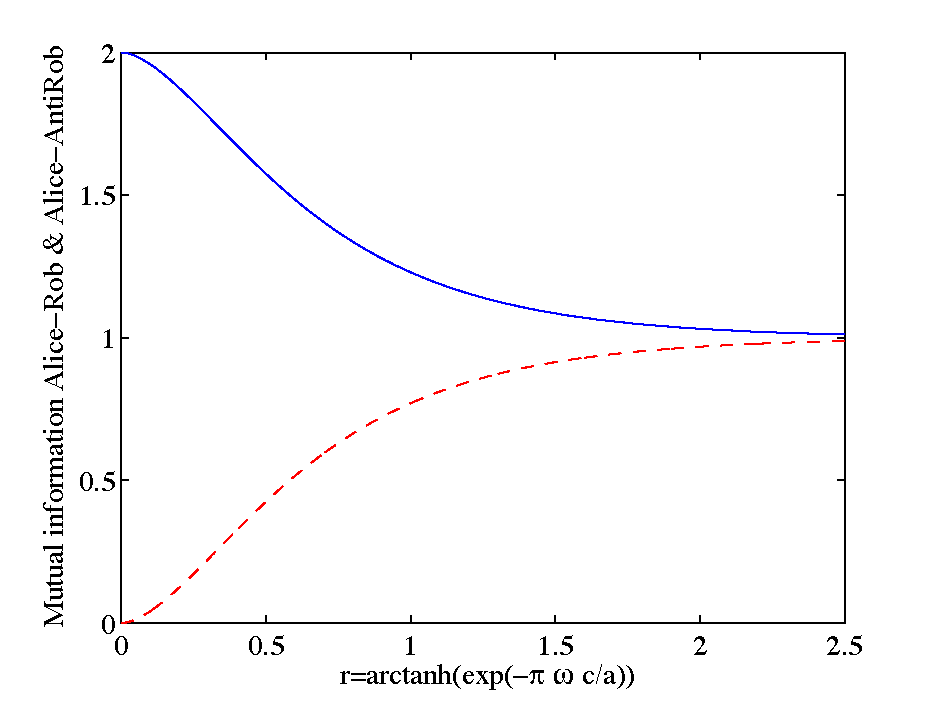
\includegraphics[width=.85\textwidth]{mutuARAARbos2}
\end{center}
\caption{ Scalar field: Mutual information conservation law for Alice-Rob and Alice-AntiRob. Blue continuous line: Mutual information $AR$, red dashed line: Mutual information $\text{A}{\bar{\text{R}}}$.}
\label{mututradeoffbos}
\end{figure}
\begin{figure}[h]
\begin{center}
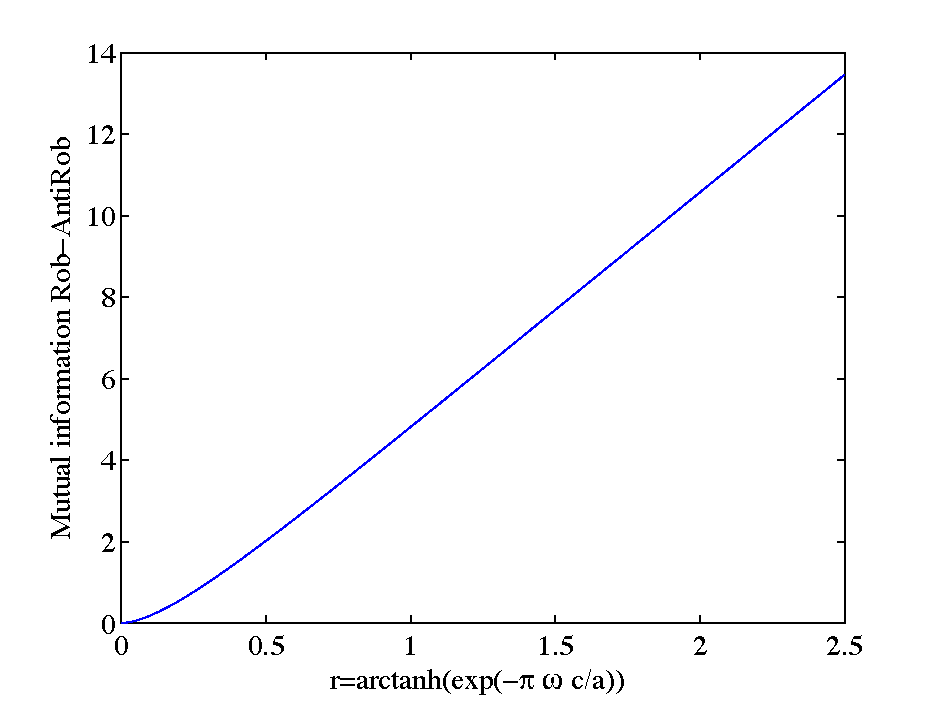
\includegraphics[width=.85\textwidth]{mutualRARbos}
\end{center}
\caption{Scalar field: Mutual information for the system Rob-AntiRob as acceleration varies.}
\label{mutuRARbos4m}
\end{figure}

\subsection{Entanglement behaviour}\label{negatsecm4}

 As we did for fermionic fields, we will compute the negativity for the scalar case.  To do so, we need the partial transpose of the bipartite density matrices \eqref{rhoars14m}, \eqref{rhoa-rs14m} and \eqref{rhor-rs14m}, which we will notate as $\eta^\text{AR}_\text{b}$, $\eta^{\text{A}{\bar{\text{R}}}}_\text{b}$ and $\eta^{\text{R}{\bar{\text{R}}}}_\text{b}$  respectively.
\begin{align}\label{etaARs4m}
\eta^\text{AR}_\text{b}&=\sum_{n=0}^{\infty}\frac{\tanh^{2n}r_\text{b}}{2\cosh^2 r_\text{b}}\Big[\proj{0n}{0n}+\frac{\sqrt{n+1}}{\cosh r_\text{b}}\Big(\proj{0\, n+1}{1n}\nonumber\\*
&+\proj{1 n}{0\,n+1}\Big)+\frac{n+1}{\cosh^2 r_\text{b}}\proj{1\,n+1}{1\,n+1}\Big],
\end{align}
\begin{align}\label{etaAaRs4m}
\nonumber\eta^{\text{A}{\bar{\text{R}}}}_\text{b}&=\sum_{n=0}^{\infty}\frac{\tanh^{2n}r_\text{b}}{2\cosh^2 r_\text{b}}\Big[\proj{0n}{0n}+\frac{\sqrt{n+1}}{\cosh r_\text{b}}\tanh r_\text{b}\Big(\ket{0 n}\bra{1\, n+1}\\*
&+\proj{1\, n+1}{0n}\!\Big)\!+\!\frac{n+1}{\cosh^2 r_\text{b}}\proj{1n}{1n}\!\Big],
\end{align}
\begin{equation}\label{etaRaRs4m}
\eta^{\text{R}{\bar{\text{R}}}}_\text{b}=\sum_{\substack{n=0\\m=0}}^{\infty}\frac{\tanh^{n+m}r_\text{b}}{2\cosh^2 r_\text{b}}\Big(\proj{nm}{mn}+\frac{\sqrt{n+1}\sqrt{m+1}}{\cosh^2 r_\text{b}}\proj{n+1\,m}{m+1\,n}\!\Big).
\end{equation}

In the following paragraphs we shall compute the negativity of each bipartition of the system.
 
\subsubsection{Bipartition Alice-Rob}


Excepting the diagonal element corresponding to $\proj{00}{00}$ (which forms a $1\times1$ block itself), the partial transpose of the density matrix $\rho^{A R}_\text{b} $ \eqref{etaARs4m} has a $2\times2$ block structure in the basis $\{ \ket{0\, n+1},\ket{1 n}\}$
\begin{equation}\label{blocks}
\frac{\tanh^{2n}r_\text{b}}{2\cosh^2 r_\text{b}}
\left(\!\begin{array}{cc}
\tanh^2 r_\text{b} & \dfrac{\sqrt{n+1}}{\cosh r_\text{b}}\\
\dfrac{\sqrt{n+1}}{\cosh r_\text{b}} & \dfrac{n}{\sinh^2r_\text{b}}
\end{array}\!\right).
\end{equation}
Hence, the eigenvalues of \eqref{etaARs4m} are
\begin{align}
\nonumber\lambda^1&=\frac{1}{2\cosh^2r_\text{b}},\\*
\lambda^2_n&=\frac{\tanh^{2n} r_\text{b}}{4\cosh^2 r_\text{b}}\left[\left(\frac{n}{\sinh^2r_\text{b}}+\tanh^2 r_\text{b}\right)\pm\sqrt{\left(\frac{n}{\sinh^2r_\text{b}}+\tanh^2 r_\text{b}\right)^2+\frac{4}{\cosh^2 r_\text{b}}}\right].
\end{align}
And then the negativity for this bipartition is
\begin{equation}
\mathcal{N}^\text{AR}_\text{b}\!=\!\sum_{n=0}^\infty\frac{\tanh^{2n} r_\text{b}}{4\cosh^2 r_\text{b}}\left|\!\left(\frac{n}{\sinh^2r_\text{b}}+\tanh^2 r_\text{b}\right)\!-\sqrt{\left(\frac{n}{\sinh^2r_\text{b}}+\tanh^2 r_\text{b}\right)^2\!\!+\frac{4}{\cosh^2 r_\text{b}}}\right|.
\end{equation}

Fig. \ref{negARbosfig} shows $\mathcal{N}^\text{AR}_\text{b}$ as a function of $r_\text{b}$.

\begin{figure}[h]
\begin{center}
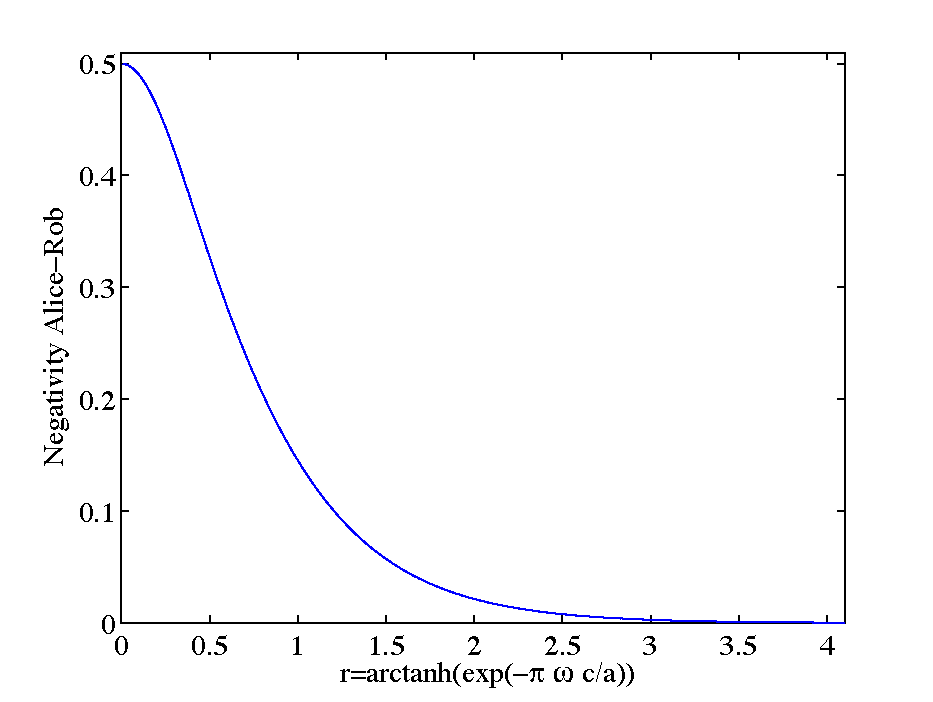
\includegraphics[width=.85\textwidth]{negARbos}
\end{center}
\caption{ Scalar field: Behaviour of the negativity for the bipartition Alice-Rob as Rob accelerates}
\label{negARbosfig}
\end{figure}

\subsubsection{Bipartition Alice-AntiRob}

Excepting the diagonal element corresponding to $\proj{10}{10}$ (which forms a $1\times1$ block itself), the partial transpose of the density matrix $\rho_\text{b}^{\text{A}{\bar{\text{R}}}}$ \eqref{etaAaRs4m} has a $2\times2$ block structure in the basis $\{ \ket{0 n},\ket{1\, n+1}\}$ 
\begin{equation}\label{blocksbosAaR}
\frac{\tanh^{2n}r_\text{b}}{2\cosh^2 r_\text{b}}
\left(\!\begin{array}{cc}
1 & \dfrac{\tanh r_\text{b}}{\cosh r_\text{b}}\sqrt{n+1}\\
\dfrac{\tanh r_\text{b}}{\cosh r_\text{b}}\sqrt{n+1} & \dfrac{\tanh^2 r_\text{b}}{\cosh^2r_\text{b}}(n+2)
\end{array}\!\right).
\end{equation}
Hence, the eigenvalues of \eqref{etaAaRs4m} are
\begin{align}
\nonumber\lambda^1&=\frac{1}{2\cosh^4 r_\text{b}},\\*
\lambda^2_n&=\frac{\tanh^{2n}r_\text{b}}{4\cosh^2 r_\text{b}}\left[\left(1+(n+2)\frac{\tanh^2 r_\text{b}}{\cosh^2 r_\text{b}}\right)\pm\sqrt{\left(1+(n+2)\frac{\tanh^2 r_\text{b}}{\cosh^2 r_\text{b}}\right)^2-\frac{4\tanh^2 r_\text{b}}{\cosh^2 r_\text{b}}}\right].
\end{align}
Therefore, the negtivity for this bipartition is always $0$, independently of the value of Rob's acceleration. This is a striking difference with the fermionic case: In the fermionic case there is an entanglement tradeoff between the partitions Alice-Rob and Alice-AntiRob but in the bosonic case all the entanglement in the first bipartition is lost while no entanglement at all is created in the A${\bar{\text{R}}}$ bipartition. We will see in chapter \ref{boundedpop} that this happens even if we consider limited occupation number bosons, therefore this is a purely statistical effect.

\subsubsection{Bipartition Rob-AntiRob}

The partial transpose of the density matrix $\rho^{\text{R}{\bar{\text{R}}}}_\text{b}$  \eqref{etaRaRs4m} has a block structure, but the blocks themselves are of different dimensions  which grow up to infinity. Because of this, negativity is not as easily computable as for the other cases, not being possible to write it in a closed form.

However it is still possible to compute the eigenvalues of \eqref{etaRaRs4m} numerically taking into account that the blocks which form the matrix are  endomorphisms which act in the subspace expanded by the basis $B_{D}=\{\ket{mn}\}$ in which $m+n=D-1=\text{constant}$, which is to say, the fisrt block acts within the subspace expanded by the basis $B_1=\{\ket{00}\}$, the second $B_2=\{\ket{01},\ket{10}\}$, the third $B_3=\{\ket{02},\ket{20},\ket{11}\}$, the fourth $B_4=\{\ket{03},\ket{30},\ket{12},\ket{21}\}$ and so forth. In this fashion, the whole matrix is an endomorphism within the subspace $\bigoplus_{i=1}^\infty S_i$ being $S_i$ the subspace (of dimension $D=i$) expanded by the basis $B_i$.

Let us denote $M_D$ the blocks which form the matrix \eqref{etaRaRs4m}, being $D$ the dimension of each block. Then its structure is
\begin{equation}\label{blockss}
M_D=\left(\!
\begin{array}{cccccccc}
0  & a_1  & 0 & 0 & \cdots & \cdots& \cdots& 0 \\
a_1 & 0 & a_2 & 0 & \cdots & \cdots& \cdots & 0\\
0 & a_2 & 0 & a_3 & \cdots & \cdots& \cdots& 0\\
0 & 0 & a_3 &0 & a_4 & \cdots& \cdots& 0\\
0 & 0 & 0 &  \ddots &\ddots &  \ddots &\cdots& 0\\
\vdots  & \vdots  & \vdots  & \vdots  & \ddots  & \ddots  & \ddots  & \vdots \\
0 & 0 & 0 &  0 &\cdots&  \ddots &0& a_{D-1}\\
0 & 0 & 0 &  0 &0&  \dots &a_{D-1}& a_{D}\\
\end{array}\!\right),
\end{equation}
which is to say, the diagonal terms are zero except for the last one, and the rest of the matrix elements are zero excepting the two diagonals on top and underneath the principal diagonal. The elements $a_n$ are defined as follows
\begin{equation}
a_{2l+1}=\frac{(\tanh r_\text{b})^{D-1}}{2\cosh^2 r_\text{b}},
\end{equation}
\begin{equation}
a_{2l}=\sqrt{D-l}\,\sqrt{l}\frac{(\tanh r_\text{b})^{D-2}}{2\cosh^4r_\text{b}}.
\end{equation}
Notice that the elements are completely different when the value of the label $n$ is odd or even.

As the whole matrix is the direct sum of the blocks
\begin{equation}
\eta_\text{b}^{\text{R}{\bar{\text{R}}}}=\bigoplus_{D=1}^\infty M_D,
\end{equation}
the eigenvalues and, specifically, the negative eigenvalues of $\eta_\text{b}^{\text{R}{\bar{\text{R}}}}$ would be the negative eigenvalues of all the blocks $M_D$ gathered togheter. It can be shown that the absolute value of the negative eigenvalues of the blocks decreases quickly as the dimension increases. Thus, the negativity $\mathcal{N}^{\text{R}{\bar{\text{R}}}}_\text{b}$ promptly converges to a finite value for a given value of $r_\text{b}$.  Fig  \ref{negaRARbos} shows the behaviour of $\mathcal{N}^{\text{R}{\bar{\text{R}}}}_\text{b}$ with $r_\text{b}$, showing that the entanglement increases unboundedly between Rob and AntiRob.

\begin{figure}[h]
\begin{center}
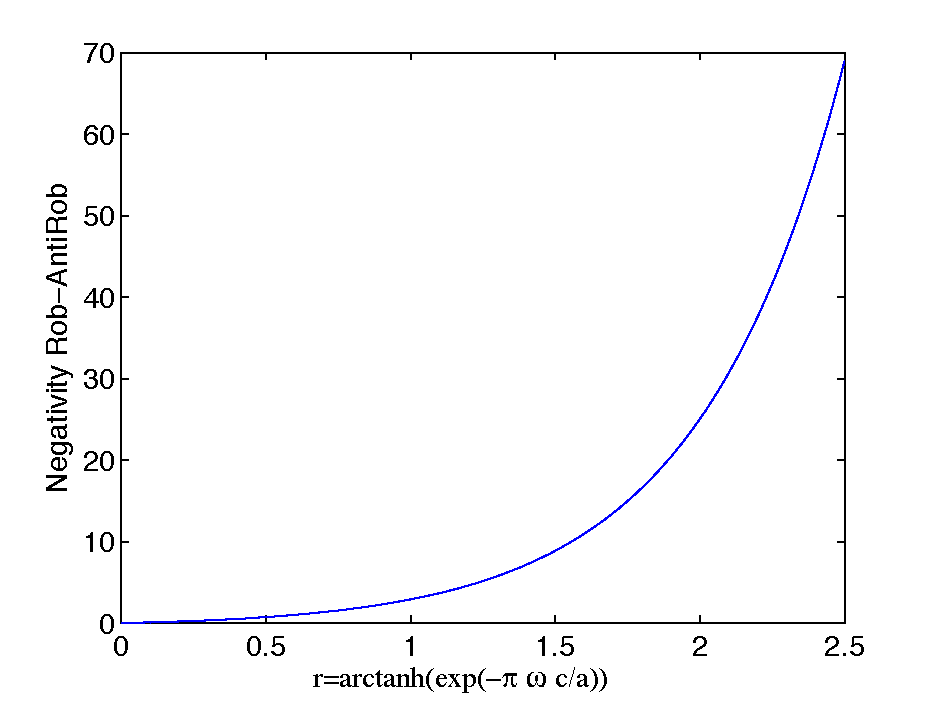
\includegraphics[width=.85\textwidth]{negaRARbos}
\caption{ Scalar field: Behaviour of the negativity for the bipartition Rob-AntiRob as Rob accelerates.}
\label{negaRARbos}
\end{center}
\end{figure}

Let us compare these results with the fermion case. First, as it was shown in \cite{AlsingSchul}, the negativity of the system Alice-Rob decreases as Rob accelerates, vanishing in the limit $a\rightarrow\infty$, instead of remaining finite as in the fermionic cases (\cite{AlsingSchul} and previous chapters of this thesis) .

What may be more surprising is the behaviour of quantum correlations of the system Alice-AntiRob. In the fermion case negativity grows monotonically from zero (for $a=0$) to a finite value (for $a=\infty$). Nevertheless, for scalars, Alice-AntiRob negativity is identically zero for all acceleration. Hence, there is no transfer of entanglement from Alice-Rob to Alice-AntiRob as it was the case for fermions. Still, correlations (classical) are not lost as it can be concluded from \eqref{conservationbos}.


Why do we obtain such loss of entanglement for the bosonic case and, conversely, this does not happen in the fermionic case? The answer is, once again, statistics. 

One could think of the infinite dimensionality of the Hilbert space for scalars (compared to the finite dimension for fermions) as the cause of this different behaviour. However we shall prove that it has to do with the bosonic nature of the field rather than with the infinite dimensionality of the Hilbert space. We will see this when we consider limited dimension bosons instead of scalars, which is to say, limiting the occupation number for the bosonic modes to a certain finite limit $N$ instead of taking $N\rightarrow\infty$. By doing so, we transform the infinite dimension Hilbert space for bosons into a finite dimension one. That is what we will do in the next chapter.

As for the bipartition Rob-AntiRob, we observe that entanglement grows unboundedly for this bipartition, conversely to the fermion case in which negativity increases up to a certain finite limit as Rob accelerates.  At first glance at Fig. \ref{mutuRARbos4m} and \ref{negaRARbos} one could think that there might be some inconsistency between the behaviour of entanglement and mutual information, as the latter grows linearly while negativity seems to grow exponentially. Since mutual information accounts for all the correlations (quantum and classical) between Rob and AntiRob, the result may appear paradoxical. However this apparently inconsistent results are due to the fact that negativity cannot be identified as the entanglement itself, but as a monotone which grows as the degree of entanglement does.  The specific functional form chosen for the monotone is not imposed by physical motivations. Actually, we could have chosen logarithmic negativity  --instead of negativity-- as our entanglement monotone since it is in fact better to be compared with mutual information due to its additivity properties \cite{logneg}. The result obtained in this case, shown in Fig. \ref{logneg2}, is that when acceleration grows both growths become linear.
\begin{figure}[h]
\begin{center}
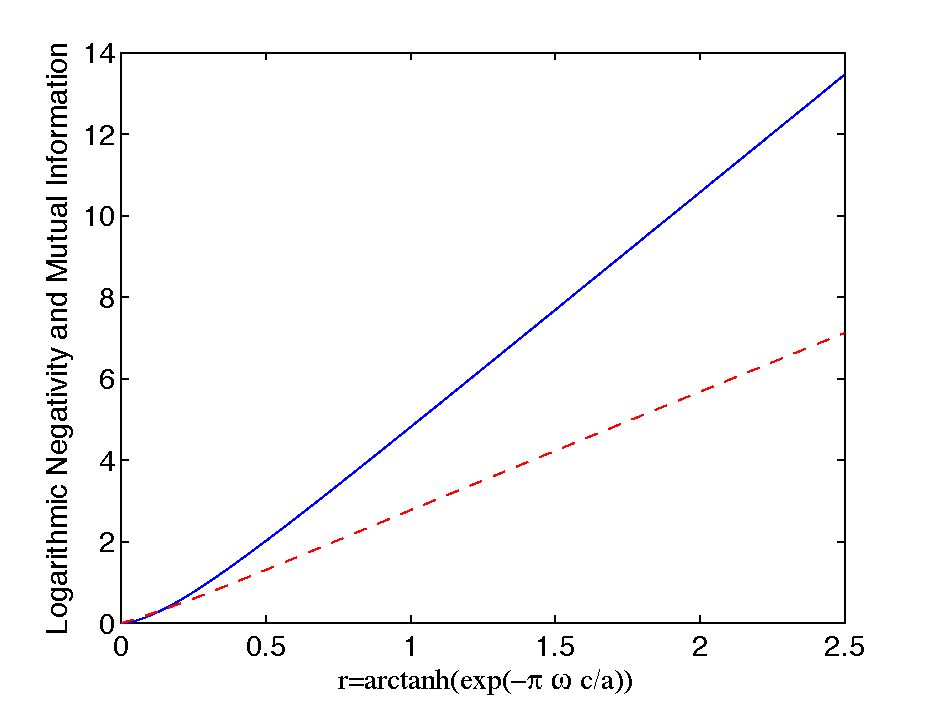
\includegraphics[width=.85\textwidth]{lognegMIRAR}
\caption{Scalar field: Comparison of growth of quantum and all (quantum+classical) correlations for the system Rob-AntiRob as acceleration increases. Quantum correlations are accounted for by logarithmic negativity (Red dashed line). This figure compares this entanglement measurement with mutual information (Blue continuous line).}
\label{logneg2}
\end{center}
\end{figure}


\section{Discussion}\label{conclusions}

This chapter focused on the bipartite correlations between different spacetime domains in the presence of an acceleration horizon. Specifically, we analyse all the possible bipartitions of an entangled system composed by an inertial observer and an accelerated one, who sees an acceleration horizon.

First of all, we have studied the relation between the entanglement behaviour of Alice-Rob and Alice-AntiRob bipartitions, which are the ones where communication is allowed. 

Here we have disclosed a great difference in the behaviour of quantum correlations for fermions and bosons. In the fermionic case we showed that, at the same time as Unruh decoherence destroys the entanglement of the system Alice-Rob, entanglement is created between Alice and AntiRob. This means that the quantum entanglement lost between Alice and the field modes in region I is gained between Alice and the modes in region II. This is expressed through the entanglement conservation law \eqref{conservationN}, which we have deduced for fermions.

Nevertheless, for bosonic states it was shown that, as acceleration increases, entanglement is quickly and completely lost between Alice and Rob while no quantum correlations are created between Alice and AntiRob. Moreover, no entanglement of any kind survives among any physical bipartition of the system in the limit $a\rightarrow\infty$ for the bosonic case. This contrasts with the fermionic case where the amount of entanglement among all the physical bipartitions of the system remains always constant.

Another remarkable result is the conservation law for mutual information for fermions \eqref{conservation1} and bosons \eqref{conservationbos} shown in  in Fig. \ref{mutuferm} and Fig. \ref{mututradeoffbos}. The detailed  behaviour is different for both cases but the same conservation law is obtained for the mutual information of the bipartitions Alice-Rob, and Alice AntiRob. Mutual information accounts for both classical and quantum correlations (despite the fact that in general there is no direct relation between negativity and mutual information). However in the bosonic case, mutual information distributes more rapidly between the  Alice-Rob and Alice-AntiRob than in the fermion case.

This result for mutual information means that correlations are always conserved for the systems Alice-Rob and Alice-AntiRob, despite the fact that quantum entanglement vanishes for the bosonic case and it is preserved (this is the effect of statistics) in the fermionic case. The fact that classical correlations behave in a similar way for fermions and bosons while quantum correlations behave so differently suggests again that the quantum entanglement which survives the infinite acceleration limit has a statistical origin, as if the information of `being fermion' cannot be killed by the presence of the horizon. Something to reflect upon: this scenario has some resemblance with the results found in quantum mechanical fermionic systems \cite{sta1} in which it was demonstrated that identical fermions systems has some degree of entanglement that is `built in' in their wavefunction.

Another difference between fermion and bosons appears when analysing the correlations between the wedges I and II. It is interesting to notice that, as the non-inertial partner accelerates, correlations between these two regions  are created. We have found that for Dirac fields these correlations, quantum and classical, grow as Rob accelerates up to a finite value at the limit $a\rightarrow\infty$. This limit is greater than the analogous limit  obtained for spinless fermions in \cite{AlsingSchul} whose Hilbert space for each mode is smaller. For the bosonic case, on the contrary, those correlations grow unboundedly, diverging when $a\rightarrow\infty$. 

